\documentclass[a4paper,12pt,titlepage = false, openany, openright, cleardoubleempty]{scrreprt} %page-size, letter-size, with title, is an article

\usepackage{color}
\usepackage{verbatim}


\usepackage{fixltx2e}

\usepackage[ngerman, english]{babel} %all inserted strings will be german
\usepackage{a4wide} %for better viewing of a4 pages
\usepackage{amsmath}
\usepackage{amssymb}

\usepackage{ntheorem}

\usepackage[T1]{fontenc} %T1-encoded fonts: auch Wörter mit Umlauten trennen
\usepackage{lmodern}
\usepackage[utf8]{inputenc} % use utf8 as encoding style

\usepackage{vmargin} %Seitenränder einstellen leichtgemacht
\usepackage{fancyhdr} %definiere einfache Headings (mindestens V 1.99c notwendig)

\usepackage{float} %to be able to insert graphics with [H] Options
\usepackage{makeidx} %so the \printindex works

\usepackage{pst-all} %pretty good drawing kit

\usepackage{listings}

\usepackage[vlined,boxed]{algorithm2e}

\usepackage[normalem]{ulem}

\usepackage{textgreek}

\usepackage{tcolorbox}
\usepackage{graphicx}

\lstset{basicstyle=\ttfamily,breaklines=true}

\usepackage{remreset} %folgende Zeilen benötigt, damit Fußnoten sich nicht zurücksetzen bei neuem Kapitel

%\usepackage[pdftex]{graphicx}

\usepackage{pdfpages}

\usepackage[pdftex,
bookmarksnumbered,
bookmarks,
bookmarksopen,
bookmarksopenlevel=1,
hypertexnames,
breaklinks,
]{hyperref}

\usepackage{xpatch}

\usepackage{xcolor}
\usepackage{titlesec}

\usepackage{svg}
%\setsvg{inkscape=inkscape -z -D,svgpath=images/}

\usepackage{scrextend}

\usepackage{enumitem}

\usepackage{tabto}

\makeatletter
\@removefromreset{footnote}{chapter}
\makeatother 



\makeatletter
\def\inverseverbatim{%
  \color{white}\normalsize
  \def\verbatim@processline{%
    {\setbox0=\hbox{\the\verbatim@line}%
    \hsize=\wd0 \the\verbatim@line\par}}%
  \@minipagetrue
  \@tempswatrue
  \@totalleftmargin\z@
  \setbox0=\vbox\bgroup \verbatim
}
\makeatother 

\makeatletter
\def\endinverseverbatim{%
  \endverbatim
  \unskip\setbox0=\lastbox
  \egroup
  \colorbox{black}{\box0}%
}
\makeatother

\makeatletter
\def\codebox{%
\color{white}\normalsize
\begin{tcolorbox}[width=\textwidth,colback={gray}, colupper=white]
}

\def\endcodebox{%
\end{tcolorbox}
}
\makeatother 

\makeatletter
\def\docunit[#1]{
\textbf{#1} 
\begingroup
\par\noindent %ab hier der Text, der eingerückt werden soll
\leftskip=1cm % Parameter anpassen
}

\makeatletter
\def\enddocunit{%
\noindent
  \par
  \endgroup
}
\makeatother



\lstset{breaklines=true}
\lstset{basicstyle=\ttfamily}
\lstset{language=Java}
\lstset{tabsize=4}

\setcounter{secnumdepth}{3}% Numerierung auch für \subsubsection
\setcounter{tocdepth}{3}% nimm auch \subsubsections ins Inhaltsverz. auf

\clubpenalty = 10000
\widowpenalty = 10000
\displaywidowpenalty = 10000

\setpapersize{A4}
\setmarginsrb{3cm}{1cm}{3cm}{1cm}{6mm}{7mm}{5mm}{15mm}

%% Stil
\parindent 0cm                     % Absatzanfang wird nicht eingerückt
\parskip1.5ex plus0.5ex minus0.5ex % Abstand zwischen zwei Absätzen

\newtheorem{Def}{Definition}

\pagestyle{fancy}
\renewcommand{\chaptermark}[1]{\markboth{\thechapter.\ #1}{}}
\fancyhf{} % clear all header and footer fields
\fancyhead[LE,RO]{{\headfont\thepage}} % left/right header for even/odd pages
\fancyhead[LO]{\headfont\nouppercase{\rightmark}} % header for left side (odd)
\fancyhead[RE]{\headfont\nouppercase{\leftmark}} % right header for even pages
\renewcommand{\headrulewidth}{0.5pt} % head rule
\renewcommand{\footrulewidth}{0pt} % no rule
% plainstyle
\fancypagestyle{plain}{%
\fancyhf{} % clear all header and footer fields
\renewcommand{\headrulewidth}{0pt}
\renewcommand{\footrulewidth}{0pt}
}


\hypersetup{
pdftitle    = {Titel},
pdfsubject  = {...},
pdfauthor   = {},
pdfkeywords = {},
colorlinks  = {false},
linkcolor   = {blue},
citecolor   = {cyan}
}
\pdfcompresslevel=9
\pdfinfo{
/CreationDate (D:2015 11 24 00 00 00) % year(4) month(2) day(2) hour(2) minute(2) second(2)
/ModDate      (D:2015 11 24 00 00 00) % modification date
}


%%%%%%%%%%%%%%%%%%%%%%%%%%%%%%%%%%%%%%
%%%%%%%%%%%%%%%%%%%%%%%%%%%%%%%%%%%%%%
%%%%%%%%%%%%%%%%%%%%%%%%%%%%%%%%%%%%%%
%%% Hier die richtige Trennung von Wörtern festlegen, die Latex sonst 
%%% falsch trennt.
%%%%%%%%%%%%%%%%%%%%%%%%%%%%%%%%%%%%%%
%%%%%%%%%%%%%%%%%%%%%%%%%%%%%%%%%%%%%%
%%%%%%%%%%%%%%%%%%%%%%%%%%%%%%%%%%%%%%
\hyphenation{Media-annotation}


\makeindex %must be before "begin{document}
\begin{document}

\renewcommand{\cleardoublepage}{}
\renewcommand{\clearpage}{}

\graphicspath{{pics/}}

\pagestyle{empty}

\pagenumbering{roman}


%%%%%%%%%%%%%%%%%%%%%%%%%%%%%%%%%%%%%%
%%% Inhaltsverzeichnis
%%%%%%%%%%%%%%%%%%%%%%%%%%%%%%%%%%%%%%

\begingroup
\titleformat{\section}[block]{\huge\bfseries\filcenter}{}{0.0em}{}
\titlespacing*{\section}{0pt}{0.0ex}{0.0ex}
\section*{MeDSpace D2RMap}
\section*{Language Specification}
\tableofcontents
\endgroup


%%%%%%%%%%%%%%%%%%%%%%%%%%%%%%%%%%%%%%
%%% Diese beiden Zeilen werden für Doppelseitigen Ausdruck benötigt und
%%% damit erst nach dem Inhaltsverzeichnis die Seiten gezählt werden.
%%%%%%%%%%%%%%%%%%%%%%%%%%%%%%%%%%%%%%
\cleardoublepage
\pagenumbering{arabic}

%%%%%%%%%%%%%%%%%%%%%%%%%%%%%%%%%%%%%%
%%% Ab hier beginnt die eigentliche Arbeit.
%%%
%%% 2 Varianten:
%%%     - entweder einzelne Kapitel mit include einbinden (bessere Übersicht)
%%%     - oder den ganzen Text einfach reinschreiben (unübersichtlich)
%%% Wie es gemacht wird spielt fürr den eigentlichen Output keine Rolle.
%%%%%%%%%%%%%%%%%%%%%%%%%%%%%%%%%%%%%%

%%% Part dient dazu, zb. die Arbeit nochmal zu Gliedern (Einleitung, Theorieteil, ...)
\part{Part}

% neues Kapitel
\chapter{Chapter}

Always make a short intro to chapters or sections.

%neue Section
\section{Section}
\label{erstesLabel}

some intro words \dots

% NICHT TIEFER ALS SUBSECTION!!!
\subsection{SubSection}
\label{zweitesLabel}

First label was set in section \ref{erstesLabel} - the second in section \ref{zweitesLabel}.

Remember: Always reference any figures or tables within the prose text!

A reference will be done like this: \cite{keyToBibEntry}

Do not cite things like Wikipedia, Slides, etc (only Books and scientific papers allowed - or W3C Recommendations \cite{w3c_example} and articles on trusted sites marked with a date and an corresponding author)

Please code URLs like this: \url{http://www.google.de}

If you name projects like A.I.R\footnote{\url{https://www.dimis.fim.uni-passau.de/iris/index.php?view=air} -- last checked: \today} or Eclipse\footnote{\url{http://www.eclipse.org/} -- last checked: \today} or whatever, use footnotes to cite the URL.

%Example Figure
\begin{figure}[H]
	\begin{center}
		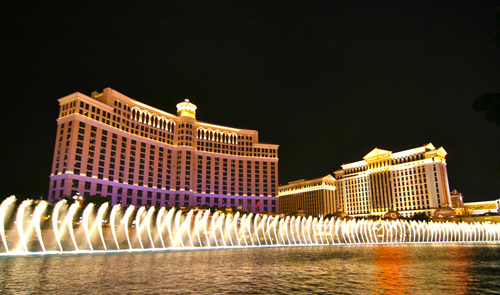
\includegraphics[width=0.75\textwidth]{holiday.png}
	\end{center}
	\caption{After the thesis it's time for holiday}
	\label{labelToRef}
\end{figure}

%Example Itemize
\begin{itemize}
	\item item 1
	\item item 2
	\item lala
\end{itemize}

%Example Description
\begin{description}
	\item[item 1] is needed in order to blabla
	\item[item 2] defines blabla
	\item[lala] lala
\end{description}

% Example Definition
\begin{Def}[Title]
\label{key}
Description \dots
\end{Def}

% Example Table
\begin{table}[H]
\begin{center}
\caption{Caption of the table}
\label{lalala}
\begin{tabular}{| l | l |}
\hline
first column & second column \\
\hline
\hline
\dots & \dots \\
\hline
\dots & \dots \\
\hline
\end{tabular}
\end{center}
\end{table}

\begin{procedure}[ht]        
\caption{Greedy Heuristic()} 
\label{greedy}        
\KwData{request profile $Q$, backends $B$} 
\KwResult{allocation schema}

sort(request profile $Q$) according cost function $c_S$ descending \; 

\ForEach{$C \in Q$}{

   \ForEach{$b \in B$}{
      \eIf{$b.free\_capacity > 0$} {
      $UNION \leftarrow b.relations \cup C.relations$\;
      $INTERSECT \leftarrow b.relations \cap C.relations$\;
      ${diff}[C,b] \leftarrow c_S(INTERSECT) - c_S(UNION)$\;
      }
      {$diff[C,b] \leftarrow -\infty$;}
   }
   
   \While{$C.rest\_workload > 0$}{
      
      $b \leftarrow b \in B \mbox{ where } diff[C,b]  \mbox{ maximal}$\;
      
      $workload\_for\_b \leftarrow \min({b.free\_capacity, C.rest\_workload})$\;
      
      $b.add(C , workload\_for\_b)$\;
      
      $C.rest\_workload \leftarrow C.rest\_workload - workload\_for\_b$\;
      
      
      ${diff}[C,b] \leftarrow -\infty$;
      
   }
}
\end{procedure}


%%%%%%%%%%%%%%%%%%%%%%%%%%%%%%%%%%%%%%
%%% Bibtex-Tool: http://jabref.sourceforge.net/
%%%%%%%%%%%%%%%%%%%%%%%%%%%%%%%%%%%%%%
\bibliographystyle{ieeetr}
\bibliography{bib.bib}
\addcontentsline{toc}{chapter}{\bibname}


\end{document}